\section{Details for Section~\ref{sec:one-shot}}

\subsection{Experimental Setup and Training Queries}
\label{app:model-data}

\paragraph{Instruction-following setup.}
\label{app:IF-setup}
Unlike the other primary-domain teachers, the instruction-following teacher is trained specifically for our experiments. Starting from DeepSeek-R1-Distill-Qwen-1.5B, we post-train the model on synthetic instruction-following tasks with programmatically checkable constraints. We use GRPO with rule-based outcome rewards that indicate whether the response satisfies the target-turn constraints. Training samples four completions per prompt at temperature \(0.9\), uses a maximum prompt length of \(4{,}096\) tokens and a maximum response length of \(16{,}384\) tokens, and optimizes with AdamW at learning rate \(1\times10^{-6}\), train batch size \(16\), and clip ratio \(0.2\). The step-600 checkpoint is used as the instruction-following teacher, improving IFBench \citep{pyatkin2026generalizing} from \(14.33\) to \(20.65\) and Multi-IF final-turn accuracy from \(20.84\) to \(28.58\).

For this domain, ``full-data'' denotes the subset sampled from UltraData-SFT-2605 \citep{ultradata-sft-2605} rather than the complete dataset, and the one-shot query is drawn at random from that subset.


\paragraph{Mathematical queries for one-shot OPD (Table~\ref{tab:one-shot-queries}, Figure~\ref{fig:probe_prompt_training_acc}).}
\label{app:training-accuracy}
We sample 8 rollouts from the untrained student for each of the first 64 queries of DAPO-Math-17K and assign difficulty by the resulting pass rate, which selects \texttt{t59} (\(8/8\)), \texttt{t22} (\(4/8\)), and \texttt{t56} (\(0/8\)) as the easy, medium, and hard queries. How often each is solved during training follows that assignment: the easy query stays near \(1.0\) throughout, the medium one rises from \(0.36\) to about \(0.89\), and the hard one is never solved in \(300\) steps, yet all three produce comparable benchmark gains in Figure~\ref{fig:probe_prompt}.

\begin{table}[t]
    \centering
    \small
    \setlength{\tabcolsep}{4pt}
    \begin{tabular}{p{0.10\textwidth}p{0.08\textwidth}p{0.74\textwidth}}
    \toprule
    Difficulty & ID & Query \\
    \midrule
    Easy & \texttt{t59} &
    In triangle \(ABC\), let \(D\) be the foot of the altitude from \(A\). Suppose that \(AD=4\), \(BD=3\), \(CD=2\), and \(AB\) is extended past \(B\) to a point \(E\) such that \(BE=5\). Determine the value of \(CE^2\). \\
    \midrule
    Medium & \texttt{t22} &
    Let \(S\) be the set of triples \((a,b,c)\) of non-negative integers such that \(a+b+c\) is even. Determine the value of
    \(\sum_{(a,b,c)\in S} \frac{1}{2^a3^b5^c}\).
    This sum can be expressed as \(\frac{m}{n}\), where \(m\) and \(n\) are relatively prime positive integers. Compute \(m+n\). \\
    \midrule
    Hard & \texttt{t56} &
    Byan is playing a game called ``raven, raven, falcon'' with his three friends. His friends sit in a circle, and Byan walks clockwise around them, tapping each friend he passes on the head and saying either ``raven'' or ``falcon,'' each with probability \(\frac{1}{2}\). The game ends when Byan has said ``falcon'' twice. The probability that one of his friends will be called a ``falcon'' twice can be expressed as \(\frac{m}{n}\), where \(m\) and \(n\) are relatively prime positive integers. Find \(100m+n\). \\
    \bottomrule
    \end{tabular}
    \caption{Mathematical queries used in the query-difficulty experiment, labelled by the student's pass rate before OPD training.}
    \label{tab:one-shot-queries}
\end{table}

\begin{figure}[t]
    \centering
    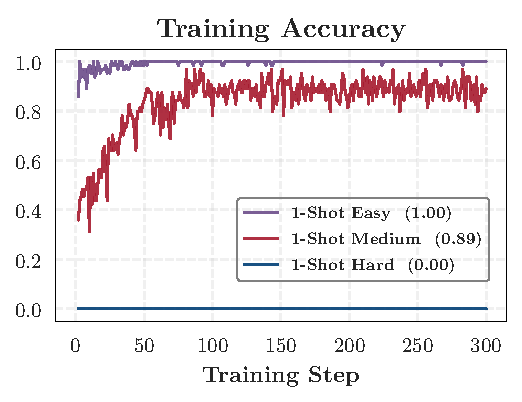
\includegraphics[width=0.45\linewidth]{figures/3A_ablations_training_acc.pdf}
    \caption{Fraction of the 64 rollouts per step that solve the training query itself, for the three queries of Table~\ref{tab:one-shot-queries}.}
    \label{fig:probe_prompt_training_acc}
\end{figure}

\paragraph{Default hyperparameters for OPD (Table~\ref{tab:opd-hyperparams}).}
Unless otherwise noted, all experiments use these defaults. The top-\(K\) row covers both objectives: the mathematical one-shot runs of Section~\ref{sec:finding-recovery} use \(K=16\), and all other experiments use the sampled-token objective.

\begin{table}[t]
\centering
\caption{Default hyperparameters for OPD.}
\label{tab:opd-hyperparams}
\small
\begin{tabular}{ll}
\toprule
\textbf{Item} & \textbf{Value} \\
\midrule
Rollout batch size      & 64 \\
Mini batch size         & 64 \\
Responses per prompt    & 1 \\
KL coefficient          & 0.0 \\
LogProb top-$K$         & 0(default) / 16 \\
Top-$K$ strategy        & Student Top-$K$ \\
Loss aggregation        & token-mean \\
Training temperature    & 1.0 \\
Top-$p$                 & 1.0 \\
Optimizer               & AdamW ($\beta_1{=}0.9$, $\beta_2{=}0.999$, wd $=0.01$) \\
Learning rate           & 1e-6 \\
Gradient clip norm      & 1.0 \\
Max prompt length       & 1024 (math); 4096 (code, IF, agentic) \\
Max response length     & 7168 (math, code, IF); 2048 (agentic) \\
\bottomrule
\end{tabular}
\end{table}


\section{Details for Section~\ref{sec:data}}

\subsection{Training-State Coverage}
\label{app:state-coverage}
\label{app:state-coverage-robustness}

\paragraph{Construction.}
Rollouts are collected by optimization step rather than at random, so that every stage of training is equally represented and the budget is comparable across settings, which run for the same number of steps: at each step from \(1\) to \(500\) of the full-data run we take \(5\) rollouts, three building the clusters and two forming full data (held-out), for \(12{,}000\) reference and \(8{,}000\) held-out states. PCA reduces these to \(50\) dimensions, retaining \(71.9\%\) of the variance, before \(K\)-means. Every evaluated setting is then measured on that same schedule, drawing \(2\) of the \(5\) rollouts at each step and accumulating over the run, so the step-\(300\) budget of \(600\) rollouts matches the held-out split. We repeat the draw \(30\) times; bands and error bars are one standard deviation over these repetitions, which reflects rollout subsampling rather than variation across trained models.

\paragraph{The ordering is stable across \(K\), reference construction, and state positions (Tables~\ref{tab:coverage-k} and~\ref{tab:coverage-reference}, Figure~\ref{fig:state-position-sensitivity}).}
Coverage depends on how finely the reference states are clustered and on which states define the clusters, so we vary both. The first table repeats the analysis at \(K\in\{50,100,200,500\}\): finer clusters lower absolute coverage, but coverage still increases from 1- to 4- to 16-shot with 16-shot close to full data. The second rebuilds the clusters from the union of \(2{,}000\) rollouts per setting instead of from full-data states alone, and the ordering survives; because states from all settings help define these pooled clusters, pooled coverage is not a recovery measure, and its rows are to be read only against each other. The figure varies the positions read from each rollout, comparing the final non-padding token and fixed absolute positions \(2{,}000\) and \(4{,}000\) against the 8 relative positions of the main analysis. All four preserve the ordering. The fixed-position variants land close to the main construction, whereas the final token gives markedly lower coverage when there are few queries, which is what one expects of a position governed by response length and termination; we therefore read 8 relative positions, which sample throughout a response of any length.

\begin{table}[t]
    \centering
    \small
    \caption{Full-data-anchored training-state coverage at step \(300\) under different cluster counts \(K\).}
    \label{tab:coverage-k}
    \begin{tabular}{lcccc}
        \toprule
        \(K\)
        & 1-shot
        & 4-shot
        & 16-shot
        & Full data (held-out) \\
        \midrule
        50  & 0.755 & 0.829 & 1.000 & 1.000 \\
        100 & 0.727 & 0.803 & 1.000 & 1.000 \\
        200 & 0.715 & 0.798 & 0.989 & 1.000 \\
        500 & 0.564 & 0.695 & 0.904 & 0.956 \\
        \bottomrule
    \end{tabular}
\end{table}

\begin{table}[t]
    \centering
    \small
    \caption{Training-state coverage under alternative cluster constructions, at \(K=200\).}
    \label{tab:coverage-reference}
    \begin{tabular}{lcccc}
        \toprule
        Reference construction
        & 1-shot
        & 4-shot
        & 16-shot
        & Full data (held-out) \\
        \midrule
        Full-data anchored
        & 0.663 & 0.773 & 0.953 & 0.998 \\
        Equal-size pooled
        & 0.750 & 0.845 & 0.958 & 0.966 \\
        \bottomrule
    \end{tabular}
\end{table}

\begin{figure}[t]
    \centering
    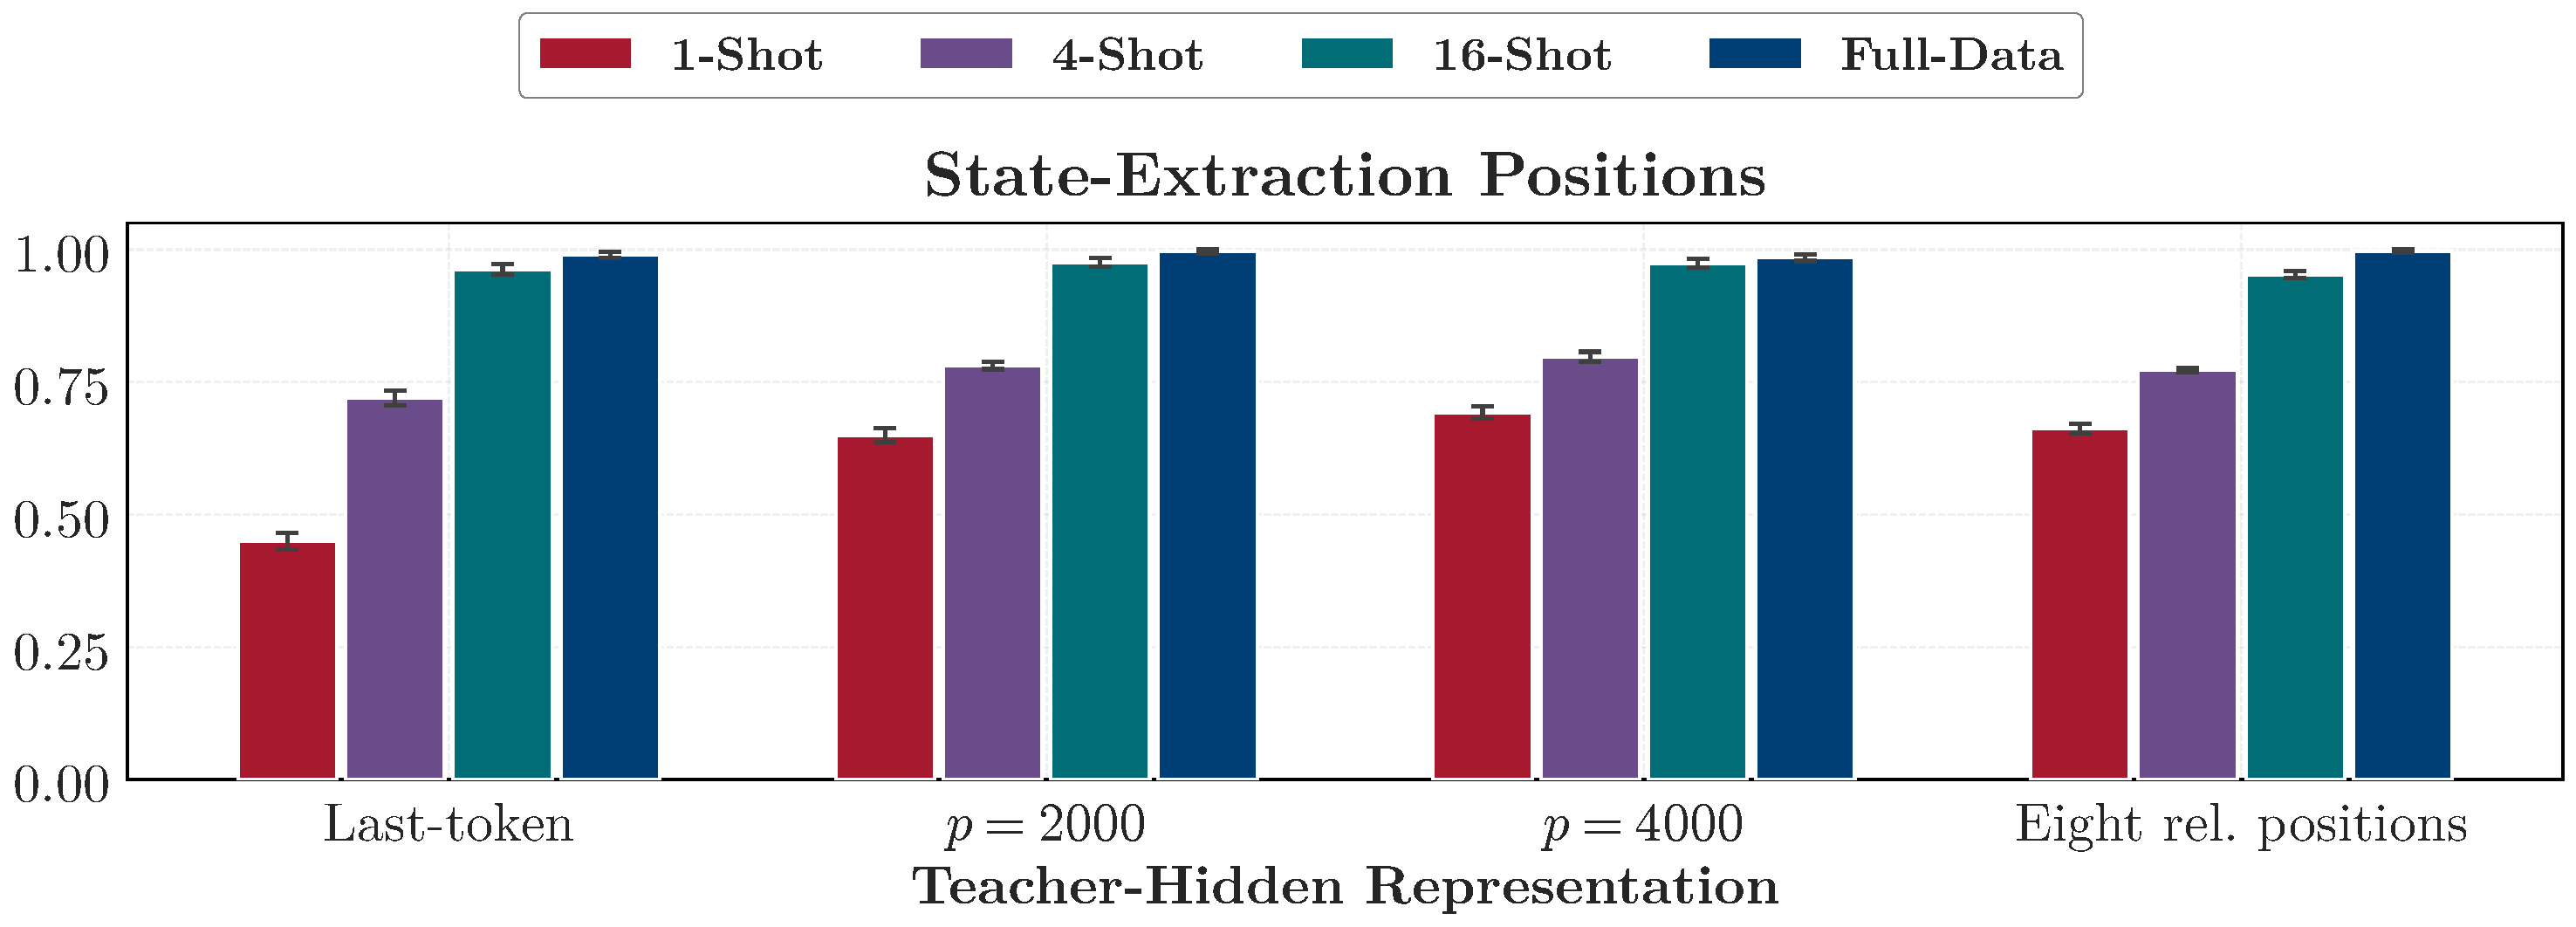
\includegraphics[width=0.85\linewidth]{figures/4A_state_extraction_positions.pdf}
    \caption{Training-state coverage under alternative state-extraction positions, at \(K=200\). Error bars show one standard deviation over rollout subsamples.}
    \label{fig:state-position-sensitivity}
\end{figure}

\paragraph{One-shot has a heavier tail of distant states, but is not separable from full data (Table~\ref{tab:reference-diagnostics}).}
Nearest-centroid assignment places a state in some cluster however far it lies from every full-data state, so coverage alone cannot tell a setting that fills the reference space thinly from one that leaves it. We therefore also measure, for each state, the mean cosine distance to its ten nearest reference states in the unreduced \(1536\)-dimensional space, and call a state off-reference when that distance exceeds the \(95\)th percentile of the held-out full-data states. One-shot OPD exceeds the threshold more often than the other settings, so its distances have a heavier upper tail. But an AUROC of \(0.552\) against held-out full-data states is close to chance, so one-shot states are not separable from full-data states as a whole.

\begin{table}[t]
    \centering
    \small
    \caption{Reference-distance diagnostics across query-set sizes. AUROC compares each setting with the held-out full-data states. The last row is the complete full-data pool, including the rollouts that built the clusters, so its exceedance rate need not equal the \(5\%\) the threshold is set at.}
    \label{tab:reference-diagnostics}
    \begin{tabular}{lccc}
        \toprule
        Setting
        & Exceedance (\%)
        & Mean distance
        & AUROC \\
        \midrule
        1-shot   & 17.2 & 0.283 & 0.552 \\
        4-shot   & 4.4  & 0.218 & 0.477 \\
        16-shot  & 3.8  & 0.231 & 0.512 \\
        Full data (all)  & 4.0  & 0.215 & 0.476 \\
        \bottomrule
    \end{tabular}
\end{table}

\subsection{Controls on the Training Data}
\label{app:fixed-count-diversity}
\label{app:schedule}

\paragraph{Diversity in 16-shot OPD (Figure~\ref{fig:fixed-count-diversity}).}
Every query on the ladder of Section~\ref{sec:state-diversity} represents a different semantic cluster, so it raises diversity and count together. Holding the count at 16 and drawing the second set from a single cluster separates them: the 16 cluster representatives reach \(70.9\) validation accuracy at step \(300\) against \(69.9\) for the single-cluster set, which is about what 4-shot OPD reaches with a quarter as many queries, and their state coverage separates the same way and does so early, \(98.9\%\) against a single-cluster set that flattens near \(76.8\%\) within \(100\) steps. Queries from one cluster keep returning the student to the part of the state space it has already seen.

\begin{figure}[t]
  \centering
  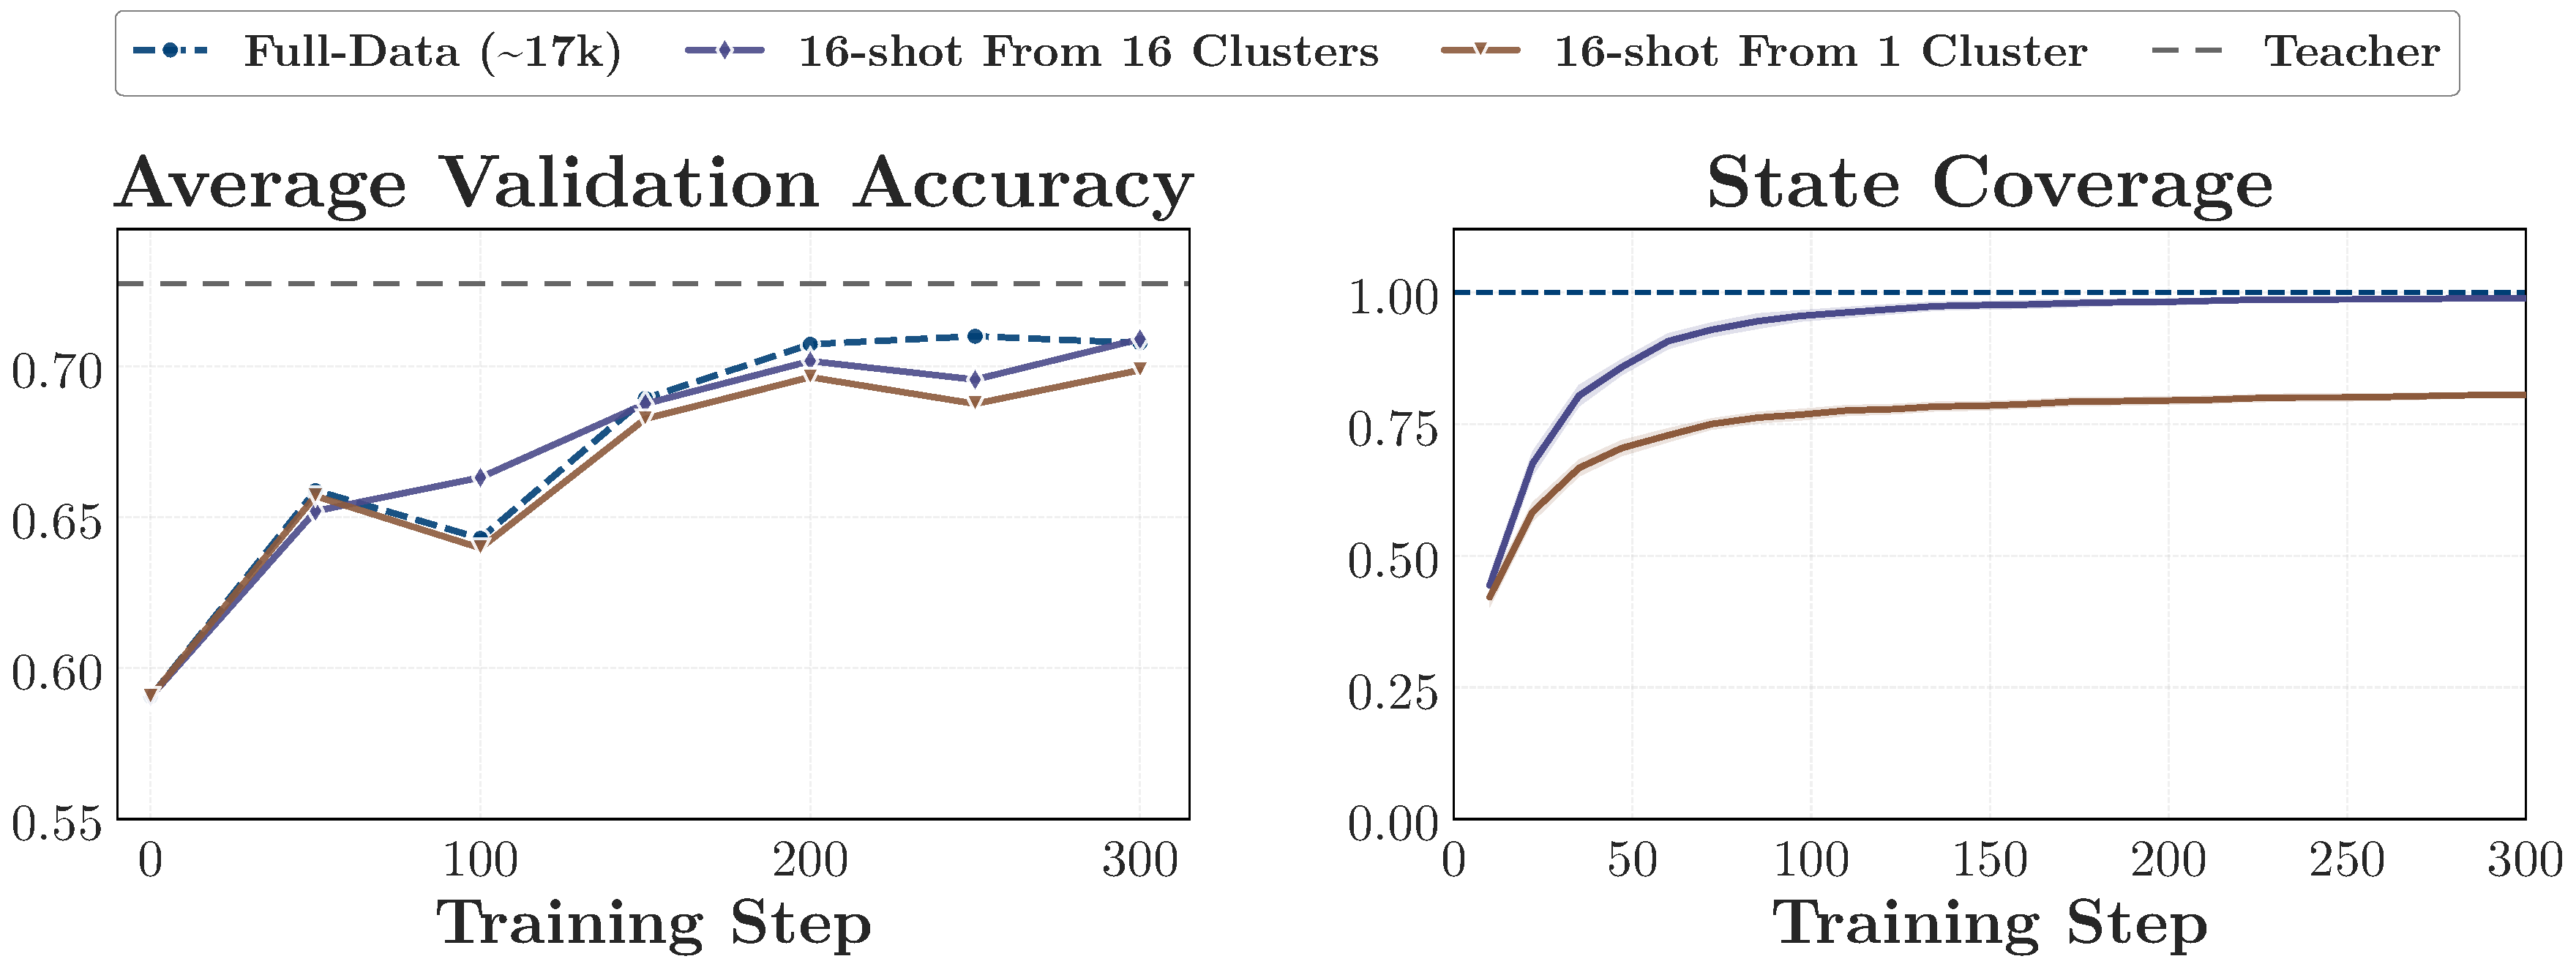
\includegraphics[width=0.75\linewidth]{figures/4A_nshot_diversity.pdf}
  \caption{Two 16-shot query sets that differ only in diversity, against full-data OPD.}
  \label{fig:fixed-count-diversity}
\end{figure}

\paragraph{Query scheduling in 2-shot OPD (Figure~\ref{fig:nshot_schedule}).}
Holding a two-query set fixed and varying only when each query is shown, the sequential schedule trains on the hard query for the first \(300\) steps of a \(600\)-step budget and on the medium query for the rest, while the mixed schedule puts \(32\) copies of each in every batch. At step \(600\) they reach \(68.8\) and \(69.1\), both above the \(67.4\) of the one-shot baseline they share, so ordering a fixed query set barely matters next to what the second query itself buys. These runs train longer than those of Section~\ref{sec:state-diversity} and take the hard query as their baseline, so neither their horizon nor their baseline is interchangeable with Figure~\ref{fig:state-diversity}.

\begin{figure}[t]
  \centering
  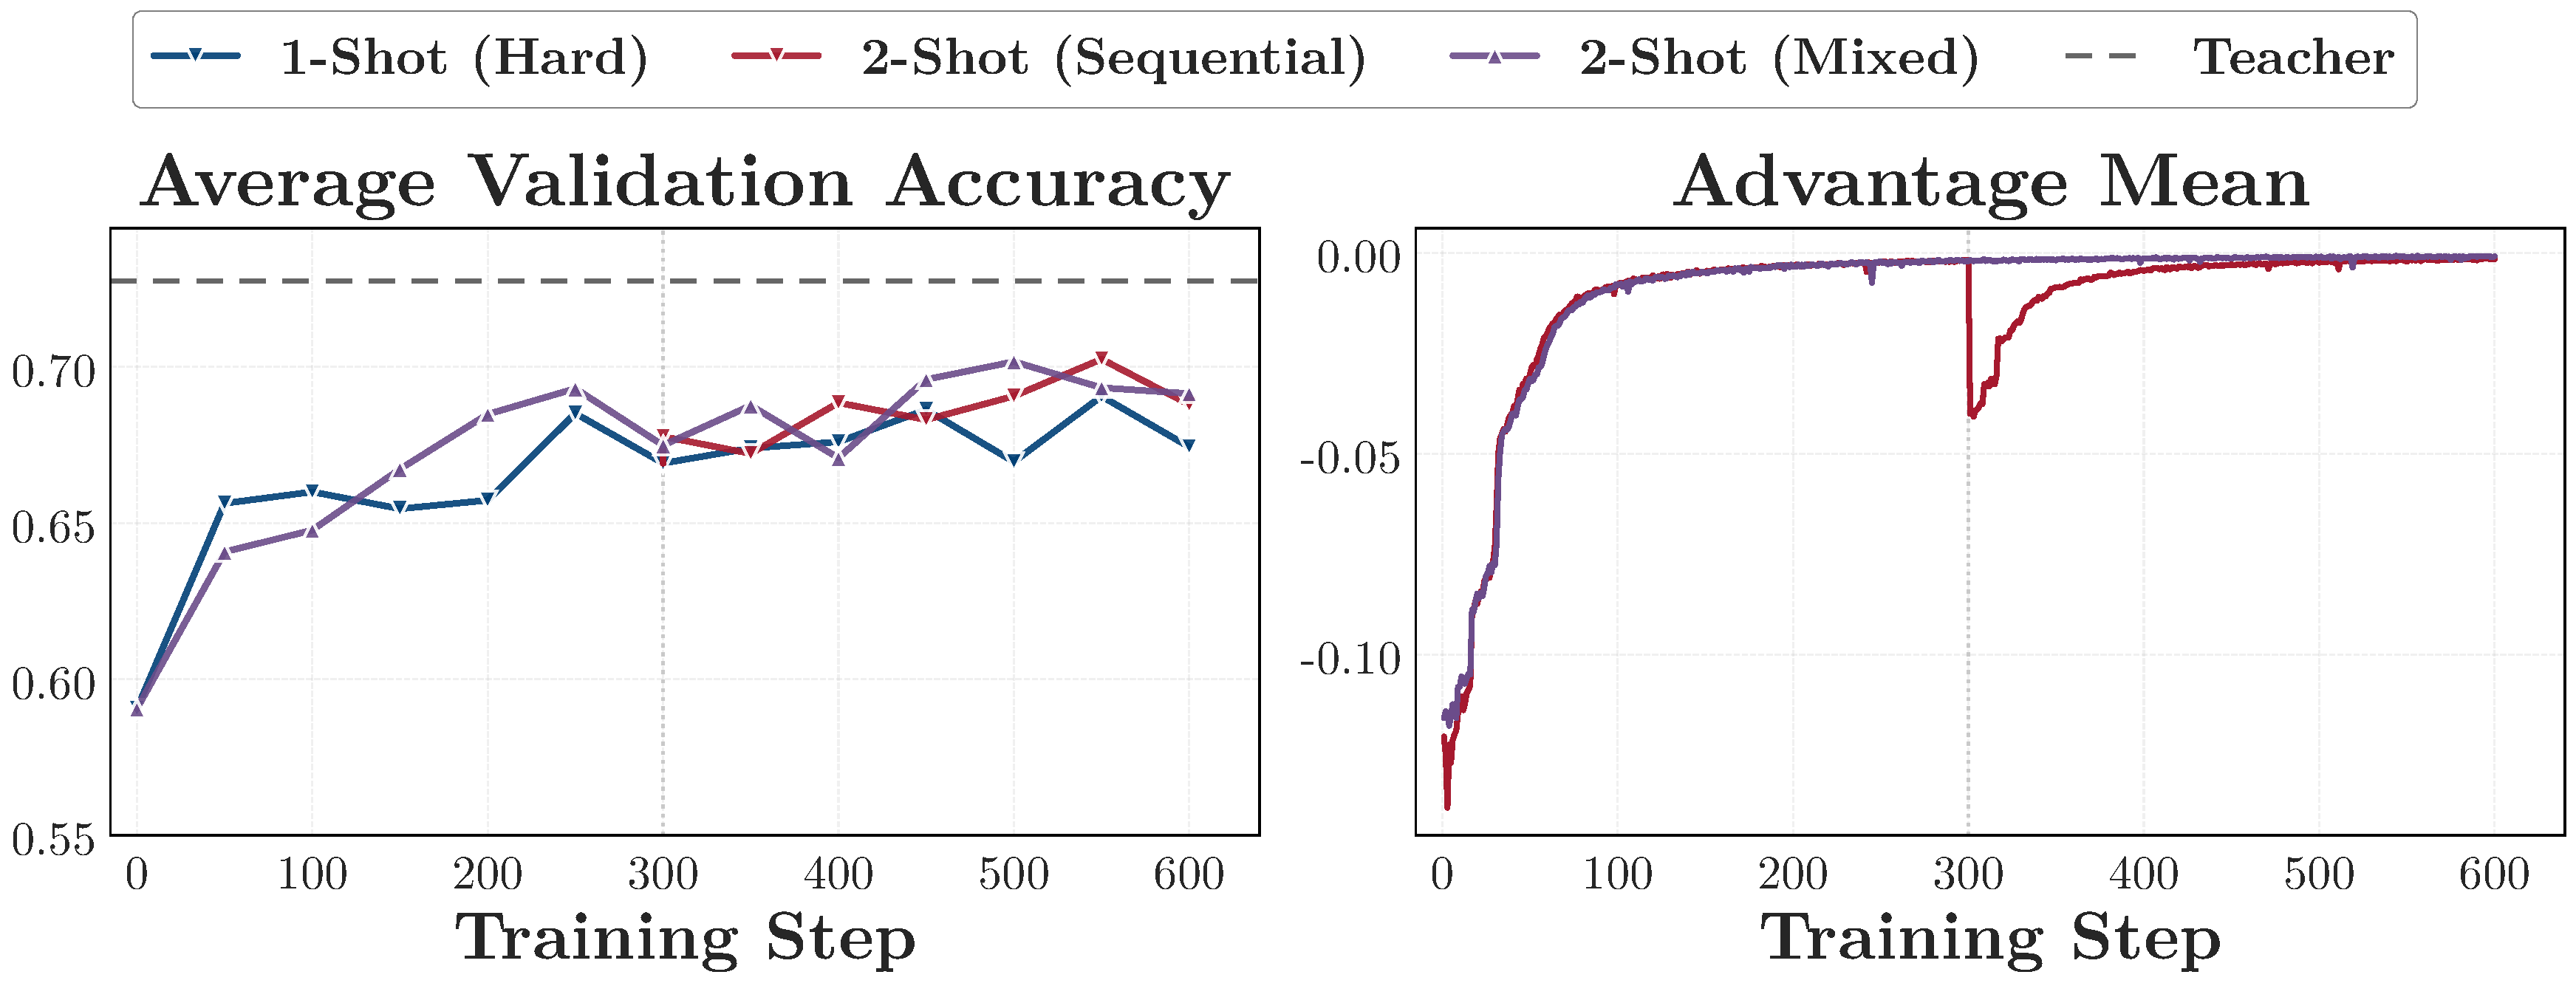
\includegraphics[width=0.75\linewidth]{figures/4A_2shot_schedule.pdf}
  \caption{Effect of query scheduling in 2-shot OPD. The vertical dotted line marks the query switch in the sequential schedule.}
  \label{fig:nshot_schedule}
\end{figure}

\section{Details for Section~\ref{sec:algorithm}}

\subsection{Estimating the Absorption Rate and the Measurement Window}
\label{app:alignment-dynamics}

Section~\ref{sec:mech-dynamics} measures under three conventions. Why each one:
\begin{itemize}[topsep=2pt, partopsep=0pt, leftmargin=13pt, itemsep=2pt, parsep=0pt]
    \item \(\boldsymbol{[t/1.4,\,1.4t]}\). A difference between adjacent steps is mostly noise once \(d\) moves slowly, so \(v_t\) is read as the slope of \(\log d\) across the endpoints of this window, using the median \(d\) near each. Only centers whose window fits inside the measured range are plotted, which is why the main text reads the rate at steps \(50\) and \(200\) rather than at step \(300\).
    \item \(\boldsymbol{d_t/d_{30}}\). Each run measures its distance on the states it visits and the four sit at different levels by step \(30\), so plotting each against its own value there lets the curves be compared by shape rather than by level.
    \item \textbf{Start at step \(30\).} Gradient clipping binds until then, and a clipped update is not the update the objective asked for: \(v_t\) inside that window measures what one \emph{fixed-size} step buys rather than what one step buys, which is why the measured rate rises there rather than falls.
\end{itemize}

Table~\ref{tab:gap-reduction} collects the readings Section~\ref{sec:mech-dynamics} quotes from this range: the proportion of the step-\(30\) distance still left at step \(300\), and the factor by which the absorption rate falls between steps \(50\) and \(200\).

\begin{table}[t]
    \centering
    \small
    \caption{Alignment dynamics over steps \(30\)--\(300\) for on-policy OPD, at the default learning rate.}
    \label{tab:gap-reduction}
    \begin{tabular}{lcccc}
        \toprule
        Setting (queries) & 1 & 4 & 16 & Full data \\
        \midrule
        \(d_{300}/d_{30}\) & 0.16 & 0.17 & 0.18 & 0.22 \\
        \(v_{50}/v_{200}\) & 5.6 & 5.2 & 4.2 & 6.4 \\
        \bottomrule
    \end{tabular}
\end{table}

\subsection{The Learning Rate Rescales the Step Axis}
\label{app:lr-sensitivity}

We repeat on-policy one-shot OPD at half, the default, and twice the default learning rate, holding every other setting fixed, and read all three over the same \(300\) steps as Section~\ref{sec:mech-dynamics}.

\begin{figure}[t]
    \centering
    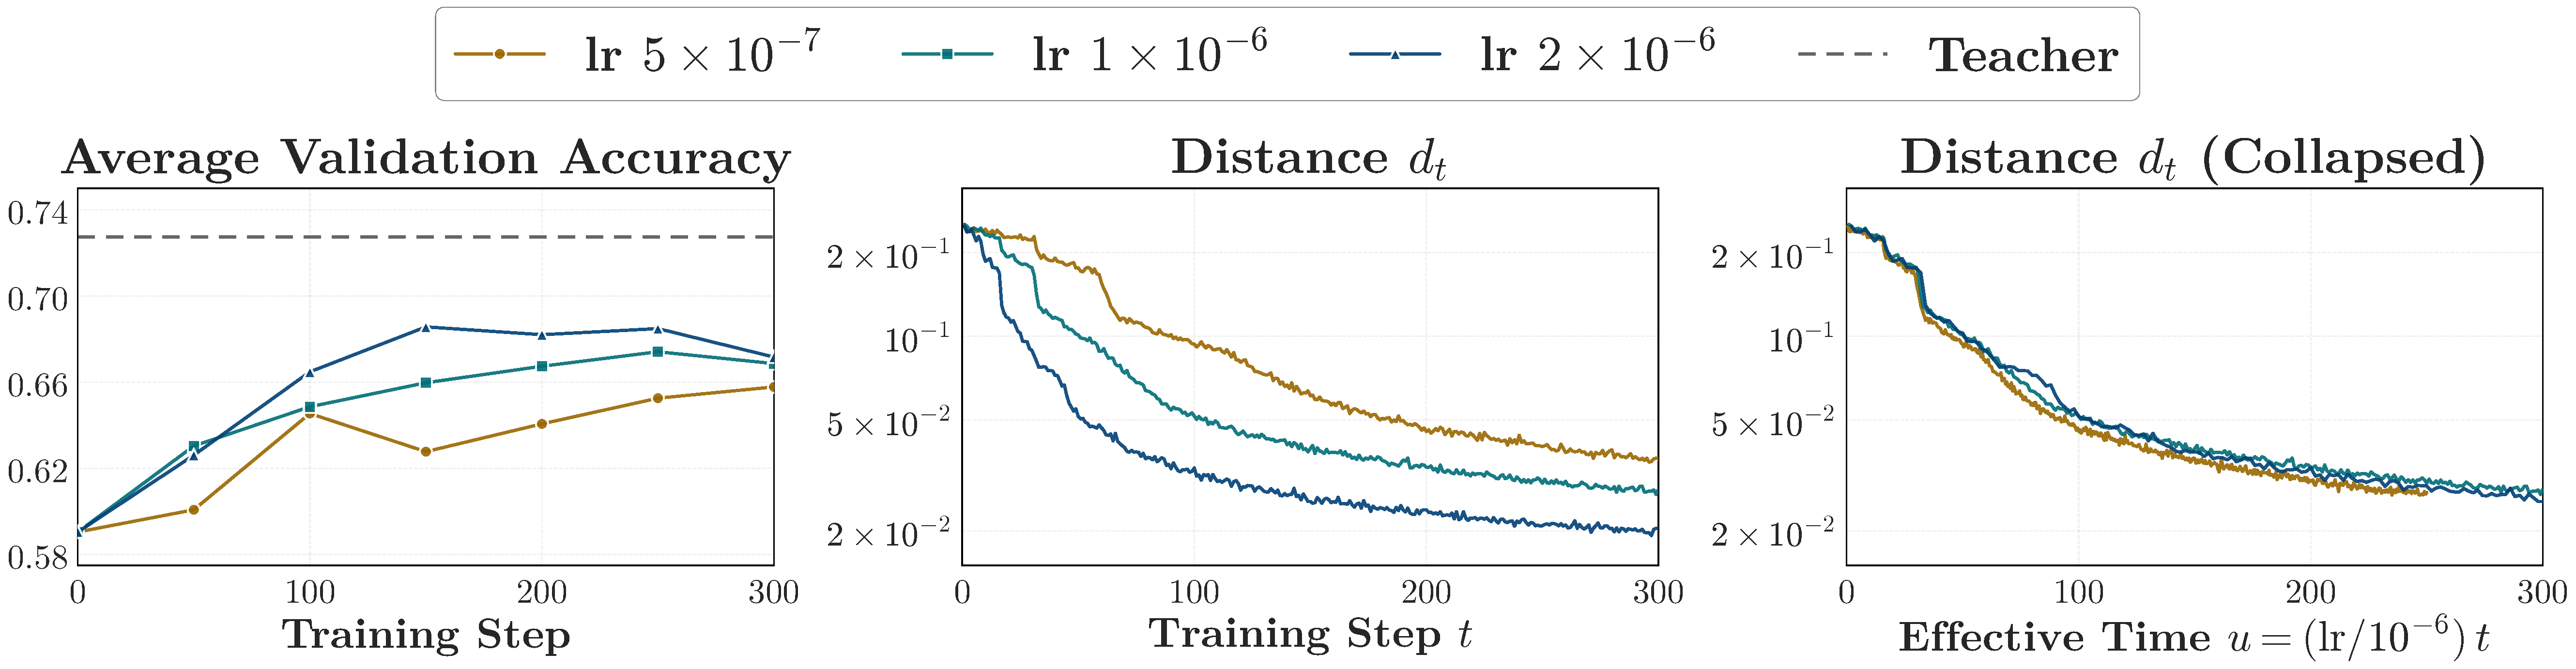
\includegraphics[width=\linewidth]{figures/5A_lr_collapse_v2.pdf}
    \caption{Validation accuracy and teacher--student distance for one-shot OPD at half, one, and twice the default learning rate. Distance is on a logarithmic vertical axis against linear time.}
    \label{fig:lr-sensitivity}
\end{figure}

\paragraph{The learning rate rescales the step axis and leaves the slowdown untouched.}
A larger learning rate reaches any given distance sooner, the three curves separated by roughly the ratio of the learning rates (Figure~\ref{fig:lr-sensitivity}). Changing the horizontal axis from the step \(t\) to \(u=(\mathrm{lr}/10^{-6})\,t\) brings them onto one curve: the spread between the three runs narrows from about \(2.2\times\) to about \(1.1\times\). The learning rate therefore sets only how fast a run moves along that one curve, not the shape of the curve itself. It bends flatter as it goes, just as the four query settings of Section~\ref{sec:mech-dynamics} do against the step count. A proportionally larger learning rate therefore shortens the run proportionally, over the fourfold range we tested, without reaching whatever makes alignment slow in the first place.


\section{Details for Section~\ref{sec:mopd}}
Table~\ref{tab:mopd-hyperparams} shows the default hyperparameters for MOPD.

\begin{table}[!ht]
\centering
\caption{Default hyperparameters for MOPD (multi-teacher on-policy distillation).}
\label{tab:mopd-hyperparams}
\small
\begin{tabular}{ll}
\toprule
\textbf{Item} & \textbf{Value} \\
\midrule
Number of teachers      & 3 (math / code / IF) \\
LogProb top-$k$         & 0  \\
KL coefficient          & 0.0 \\
Loss aggregation        & seq-mean-token-mean \\
\midrule
Rollout batch size      & 64 \\
Mini batch size         & 64 \\
Responses per prompt    & 1 \\
Training temperature    & 1.0 \\
Top-$p$                 & 1.0 \\
\midrule
Optimizer               & AdamW ($\beta_1{=}0.9$, $\beta_2{=}0.999$, wd $=0.01$) \\
Learning rate           & 1e-6 \\
Gradient clipping       & 1.0 \\
\midrule
Max prompt length       & 4096 \\
Max response length     & 7680 \\
\bottomrule
\end{tabular}
\end{table}


\section{Details for Section~\ref{sec:discussion}}

\subsection{Template and WildChat OPD in Code Generation}
\label{app:template-code}

Section~\ref{sec:template} reports the four input conditions in mathematics. Here we report the same four in code generation.

\paragraph{Setup.}
The student is R1-Distill-1.5B, the teacher DeepCoder-1.5B-Preview~\citep{deepcoder2025}, and the baseline full-data OPD on TACO~\citep{li2023taco}. The base template, the system template, and the WildChat queries are exactly those of Section~\ref{sec:template}; the system template's one-line instruction is the competitive-programming instruction of Figure~\ref{fig:template-examples}b. We evaluate on LiveCodeBench v6 under avg@3.

\begin{figure}[!htb]
  \centering
  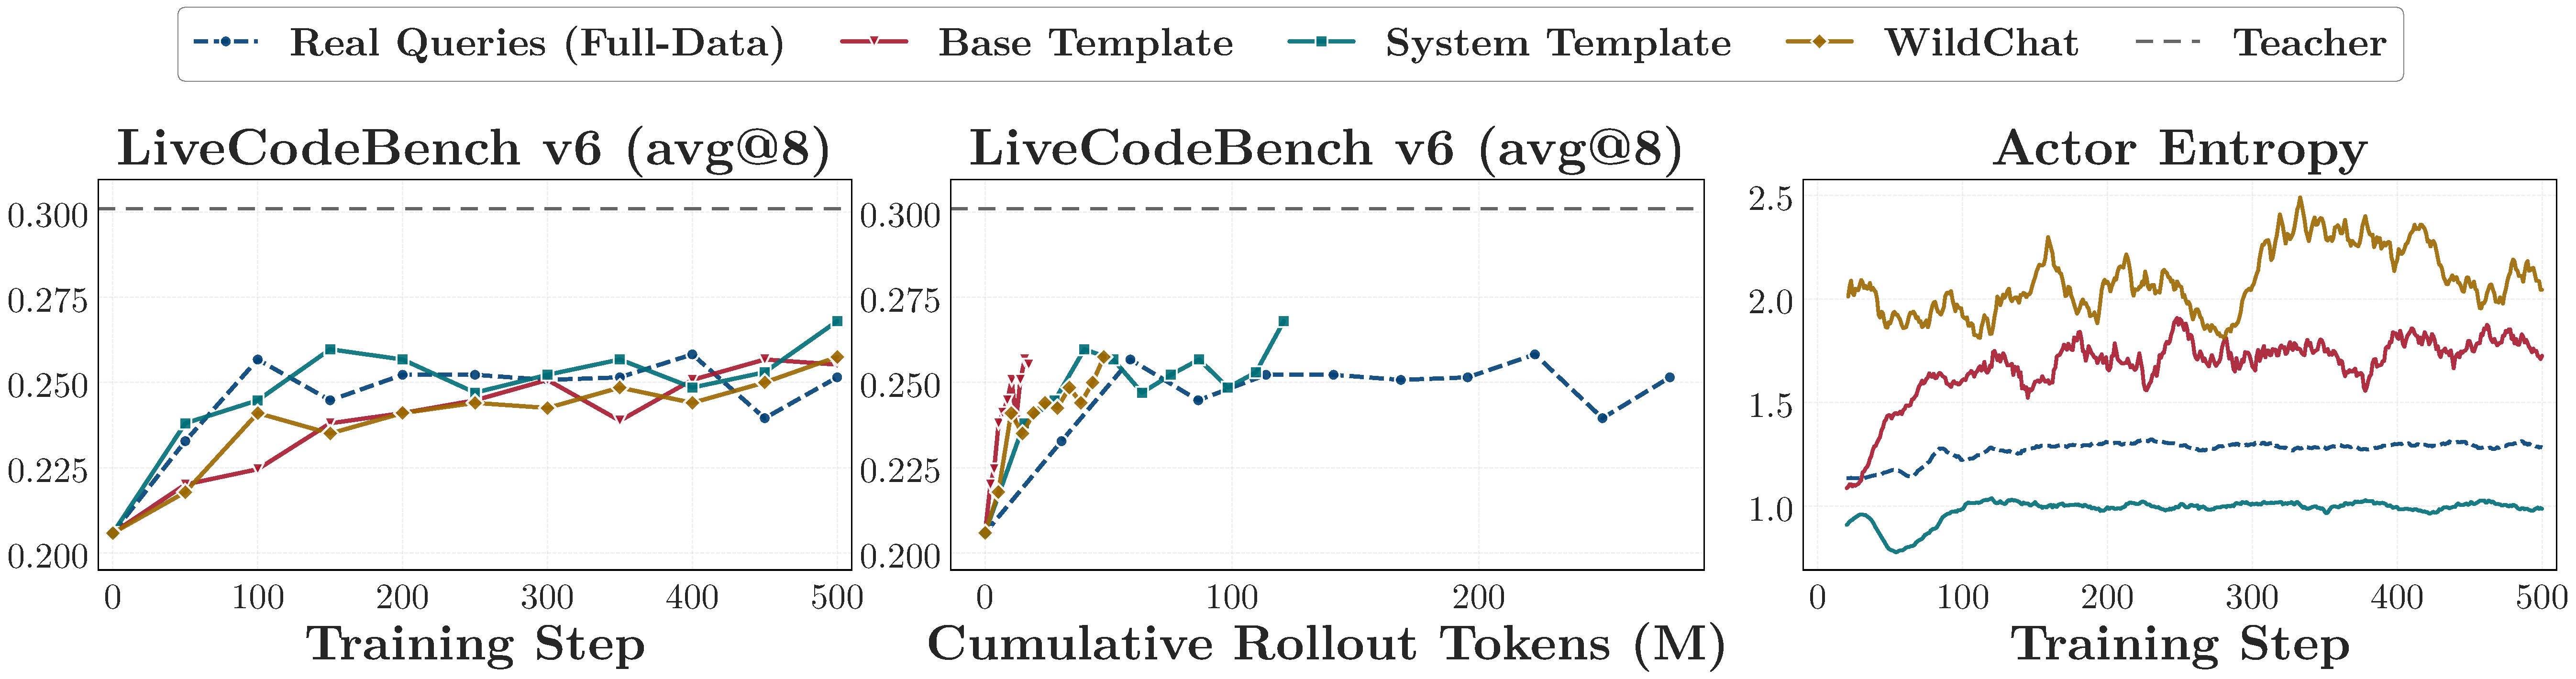
\includegraphics[width=\textwidth]{figures/7A_template_wildchat_code.pdf}
  \caption{Validation accuracy and actor entropy for code-generation OPD.
  % trained on the real training set, on a content-light template, or on general-domain WildChat queries.
  }
  \label{fig:template-wildchat-code}
\end{figure}

\paragraph{Results.}
Figure~\ref{fig:template-wildchat-code} shows the four conditions ending within \(1.7\) points of one another, and the token accounting separating them much further than the step accounting does: over the same \(500\) steps the baseline spends \(277\)M rollout tokens against \(18\)M for the base template, with the other two in between. Actor entropy orders the conditions exactly as it does in mathematics, with WildChat highest and the system template lowest. The one difference is that no condition falls behind here, whereas WildChat costs about a point in mathematics.


